\subsection{Security assessment}
We intitialy identified our assets by looking at which parts of our program might be vulnerable and of value to an intruder, 
we used the OWASP top 10 web application security risk \cite{owasp-top-10} to identify sources of threats and from these we constructed risk scenarios to get a initial overview of the risks.

After having identified risks, we used this information during Risk analysis to create a risk matrix and discuss possible solutions for the different threats. 


\begin{wrapfigure}{R}{0.38\paperwidth}
    \hspace*{0.35in}
    \makebox[0.35\paperwidth][c]{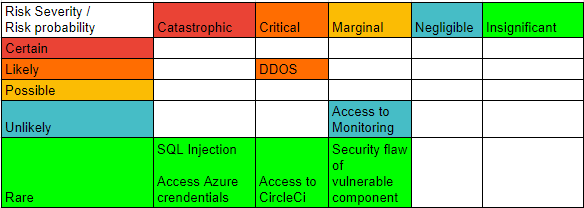
\includegraphics[width=0.43\paperwidth]{RiskAssessmentMatrix.png}}%
    \caption{Risk matrix}
    \label{fig:Risk-matrix}
\end{wrapfigure}

Some of the threats like SQL Injection and vulnerable or outdated dependencies were resolved by using an ORM \cite{gorm} as middleware for the database to clean user input and static analysis tools integrated with our pipepline like Snyk \cite{snyk} checking for vulnerable dependencies.

After risk analysis we used two vulnerability scanners OWASP ZAP \cite{owasp-zap} and Metasploit \cite{metasploit} WMAP \cite{metasploit-wmap} to test our system for vulnerabilities targeting our root endpoint \cite{minitwit-root-endpoint}.
We tried to add an extra middleware beside our CORS middleware to handle vulnerabilities flagged by the scanners, but we did not want to invest a lot of time and resources into it as we investigated the potential risks and realised they were just warnings and did not apply in our case.
We dealt with one of our risk scenarios regarding monitoring, by ensuring changes to the dashboard were only accessible through code.

Read more in our security session notes \cite{repo:security-session-notes}.
